% Customisable fields and text areas start with % >> below.
% Lines starting with the comment character (%) are normally removed before release outside the collaboration, but not those 
% comments ending lines

% svn info. These are modified by svn at checkout time.
% The last version of these macros found before the maketitle will be the one on the front page,
% so only the main file is tracked.
% Do not edit by hand!
\RCS$Revision: 207461 $
\RCS$HeadURL: svn+ssh://snarayan@svn.cern.ch/reps/tdr2/notes/IN-14-XXX/trunk/IN-14-XXX.tex$
\RCS$Id: IN-14-XXX.tex 207461 2013-09-18 14:56:50Z tapper $
\newcommand{\Na}{N_\text{accesses}}
\newcommand{\Nf}{N_\text{files}}
\newcommand{\Nr}{\langle N_\text{replicas}\rangle}
%%%%%%%%%%%%% ptdr definitions %%%%%%%%%%%%%%%%%%%%%
%\input{ptdr-definitions} %These have been replaced by the equivalent style file
%%%%%%%%%%%%%%%  Title page %%%%%%%%%%%%%%%%%%%%%%%%
%%%%%%%%%%%%% local definitions %%%%%%%%%%%%%%%%%%%%%
% This allows for switching between one column and two column (cms@external) layouts
% The widths should  be modified for your particular figures. You'll need additional copies if you have more than one standard figure size.
\newlength\cmsFigWidth
\ifthenelse{\boolean{cms@external}}{\setlength\cmsFigWidth{0.85\columnwidth}}{\setlength\cmsFigWidth{0.4\textwidth}}
\ifthenelse{\boolean{cms@external}}{\providecommand{\cmsLeft}{top}}{\providecommand{\cmsLeft}{left}}
\ifthenelse{\boolean{cms@external}}{\providecommand{\cmsRight}{bottom}}{\providecommand{\cmsRight}{right}}
%%%%%%%%%%%%% local definitions %%%%%%%%%%%%%%%%%%%%%
\input{commands.tex}
%%%%%%%%%%%%%%%  Title page %%%%%%%%%%%%%%%%%%%%%%%%
\cmsNoteHeader{IN 2014/XXX} % This is over-written in the CMS environment: useful as preprint no. for export versions
% >> Title: please make sure that the non-TeX equivalent is in PDFTitle below
\title{Popularity Metrics of Dynamically-Managed Datasets}

% >> Authors
%Author is always "The CMS Collaboration" for PAS and papers, so author, etc, below will be ignored in those cases
%For multiple affiliations, create an address entry for the combination
\address[MIT]{Massachusetts Institute of Technology}

\author[MIT]{S. Narayanan}
\author[MIT]{M. Goncharov}
\author[MIT]{C. Paus}

% >> Date
% The date is in yyyy/mm/dd format. Today has been
% redefined to match, but if the date needs to be fixed, please write it in this fashion.
% For papers and PAS, \today is taken as the date the head file (this one) was last modified according to svn: see the RCS Id string above.
% For the final version it is best to "touch" the head file to make sure it has the latest date.
\date{\today}

% >> Abstract
% Abstract processing:
% 1. **DO NOT use \include or \input** to include the abstract: our abstract extractor will not search through other files than this one.
% 2. **DO NOT use %**                  to comment out sections of the abstract: the extractor will still grab those lines (and they won't be comments any longer!).
% 3. **DO NOT use tex macros**         in the abstract: External TeX parsers used on the abstract don't understand them.
\abstract{
CMS data is ordered in datasets, which have some common properties and are usually analyzed together. As data taking progresses and Monte Carlo tools improve, datasets are often replaced and site administrators have to identify and delete out-dated datasets. Dynamic Data Management is a novel method to automatically manage the distribution and deletion of datasets. In this note, we describe a metric of DDM performance, based on the number of user requests per dataset replica.
}

% >> PDF Metadata
% Do not comment out the following hypersetup lines (metadata). They will disappear in NODRAFT mode and are needed by CDS.
% Also: make sure that the values of the metadata items are sensible. For APS submissions, they are automatically converted to APS keywords.
\hypersetup{%
pdfauthor={S. Narayanan, M. Goncharov, C. Paus},%
pdftitle={Popularity Metrics of Dynamically-Managed Datasets},%
pdfsubject={CMS},%
pdfkeywords={CMS, Dynamic Data Management, popularity}}

\maketitle %maketitle comes after all the front information has been supplied

\tableofcontents
% >> Text
%%%%%%%%%%%%%%%%%%%%%%%%%%%%%%%%  Begin text %%%%%%%%%%%%%%%%%%%%%%%%%%%%%
%% **DO NOT REMOVE THE BIBLIOGRAPHY** which is located before the appendix.
%% You can take the text between here and the bibiliography as an example which you should replace with the actual text of your document.
%% If you include other TeX files, be sure to use "\input{filename}" rather than "\input filename".
%% The latter works for you, but our parser looks for the braces and will break when uploading the document.
%%%%%%%%%%%%%%%

\section{Introduction}\label{sec:introduction}
Dynamic Data Management currently manages a pool of approximately 20 PB across several Tier 2 and Tier 1 sites. If a dataset is very popular, it will be replicated at several sites. On the other hand, we delete replicas of unpopular datasets, as long as it is not the last copy. If a dataset is declared deprecated, all copies will be deleted.  A good measure of the performance of this algorithm is the number of accesses per replica. If, for a given dataset, this number is very large, then the dataset is not sufficiently replicated. On the other hand, if it is very small for many datasets, then we are maintaining too many copies of unused datasets. To make popularity plots as shown in Figure~\ref{fig:usage}, four attributes are computed for each dataset: number of accesses, size on disk, number of files, and average number of replicas.

\begin{figure}[htbp]
    \centering
    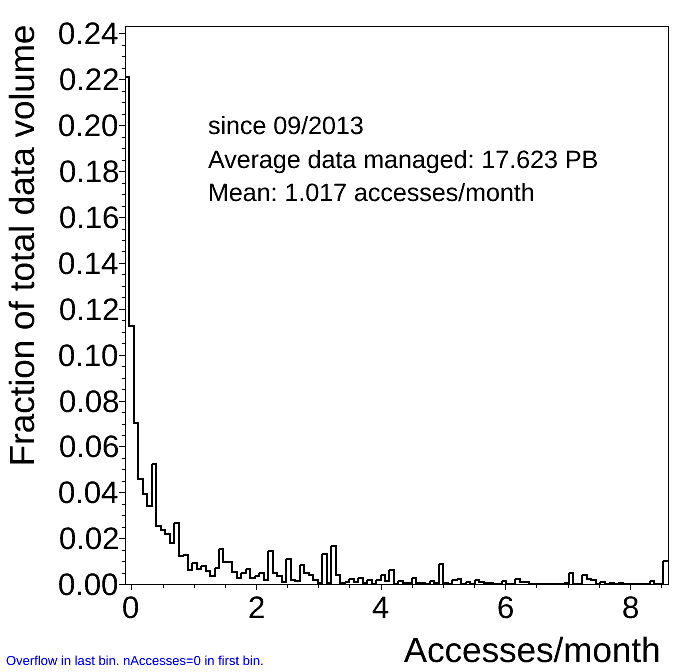
\includegraphics[width=0.45\textwidth]{plots/analysisOps_usage.png}
    \caption{Dataset usage plot for the time interval $[09/2013,\text{present}]$. Only datasets in AnalysisOps are included.}
    \label{fig:usage}
\end{figure}

% In order to identify 
% the very few, rare events that are clear signatures of new physics in our detector, we must optimally use the available 
% computing resources. The computing challenge will become harder with time, as the amount of collected data will increase 
% substantially in the years to come. The schedule at present foresees two major data taking phases - Run-II and Run-III - 
% which have the following characteristics (Run-I is also shown for comparison):

% \begin{itemize}
% 	\item Run-I: 2010-2012, nominal collision energy 7(8) TeV, accumulated data \\ 50 PB (5(20) \fbinv); 
% 	\item Run-II: 2015-2017, nominal collision energy 13 TeV, accumulated data \\ 200 PB ($\sim$ 100 \fbinv); 
%	\item Run-III: 2019-2021, nominal collision energy 14 TeV, accumulated data \\ 400 PB ($\sim$ 300 \fbinv). 
% \end{itemize}
% The numbers are staggering and while computing resources will grow and algorithmic adjustments will be made as well, it is 
% obvious that an optimization of the present system is going to have a major impact on this endeavor.

% CMS is now proposing to make best use of our computing resources by employing a novel way of managing the data distribution, based on a dynamic system that will be able to optimize the performance using a number of different system metrics.
% The plan is to treat all CMS computing sites as a network of massive caches. The optimization of the CMS data distribution in these caches is a challenging task because the system contains order of 50 geographically separated computing centers of quite different properties, and the computing tasks to be performed on them cover a wide parameter space in terms of their computing requirements. Considering the complexity of the optimization problem with perfectly working components and further including component failures into the task it is clear that there is no analytic solution and machine learning algorithms seem a great candidate to achieve a reliable and - once properly trained - low maintenance solution.

% While this is a long term project that is involving the large computing community of CMS, the MIT HEP computing group has been pioneering techniques to perform 
% automated data management at our local facilities, and here we document the core functionalities of the system that we designed, 
% translated into software, tested and put into production.


\section{Dataset attributes}

\subsection{Computing average $N_\text{replicas}$}\label{sec:replicas}

Phedex directly provides us with the current locations of all datasets. However, this information is not directly available for the past. Thus, Phedex transfer and deletion histories are used to infer the presence of a dataset on a site. The histories are `sanitized' to remove self-inconsistent entries such as the transfer of a dataset to a site on which it already exists (it is assumed that each site can only contain one copy of a dataset). If there is no Phedex history for a given dataset on a given site, but we know that the dataset is currently on that site, then it is assumed to have existed since its creation time (which is determined using DAS). 

Having collected this information, $\Nr$ can be computed for a given time interval $[t_0,t_1]$. Then, summing over the sites:
\begin{equation}
\Nr = \sum_{S\in \text{sites}} \dfrac{\text{time on }S\text{ during }[t_0,t_1]}{t_1-t_0}
\end{equation}
This gives the average number of replicas of a dataset in a specific time interval. 

\subsection{Computing $\Na$, $\text{size}$, and $N_\text{files}$}\label{sec:othervars}
The remaining variables are relatively easily calculated. The number of files and size of a dataset are gotten from DAS. It should be noted that we assume each replica is a ``full'' replica. An incomplete replica may be missing files and consequently a smaller size. We compute $\Na$ using the caches maintained by Detox. Detox is the Dynamic Data Management tool which deals with the deletion of deprecated datasets and under-utilized replicas. In order to make the latter decision, Detox keeps a local record of the number of accesses made to each replica of each dataset, derived from the popularity API. $\Na$ for a dataset is defined as the total number of accesses over all replicas of that dataset. 

\section{Filling the plot}
\subsection{Dataset selection}
Currently, we consider all datasets that are currently on, or have been on, Tier 2 sites (Tier 1s are excluded). This information is gathered from two places. First, we ask Phedex for all datasets which are currently on Tier 2s. Then, we use the \verb|deleterequests| Phedex API to determine all datasets which have been deleted during the relevant time interval. We consider all datasets in the union of these two sets. Finally, we double-check using the Phedex transfer/deletion histories that it actually was on at least one site during the interval. If the dataset passes this check, a corresponding entry is made in the histogram, as discussed below.

\subsection{Binning}

Having computed these variables for each dataset, the popularity plot may be made. The histogram is filled for each dataset by choosing the following bin-value:
\begin{equation}\dfrac{N_\text{accesses}}{N_\text{files}\cdot \Nr}\end{equation}
The factor of $\Nf$ in the denominator is due to the fact that a single request to a dataset actually consists of a series of requests to each file in the dataset. Dividing by $N_\text{files}$ ensures that this quantity is the same for small and large datasets. The entry is given weight:
\begin{equation}
\Nr\cdot \text{size}
\end{equation}
For ease of comparing plots made under different conditions, the bin-value is normalized to the length of the time interval (in Figure 1, the unit of time is months). Finally, the plot is normalized to have an integral of unity. The un-normalized integral can be thought of as a measure of ``average data volume'' during the interval, since it can be computed as:
\begin{equation}
\sum_\text{datasets} \Nr \cdot \text{size}
\end{equation}
Finally, it should be noted that there are two special bins in Figure~\ref{fig:usage}. The very last bin is the overflow bin. The very first bin contains those entries for which $\Na=0$ exactly. It is important to recall that the histogram is only filled with datasets that were on at least one site during the relevant interval. Thus, the very first bin shows the fractional volume of datasets which were on disk, but not accessed, during an interval.

% >> acknowledgements (for journal papers)
% Please include the latest version from https://twiki.cern.ch/twiki/bin/viewauth/CMS/Internal/PubAcknow.
\section*{Acknowledgements}
We congratulate our colleagues in the CERN accelerator departments for the excellent performance of the LHC and thank the technical and administrative staffs at CERN and at other CMS institutes for their contributions to the success of the CMS effort. In addition, we gratefully acknowledge the computing centres and personnel of the Worldwide LHC Computing Grid for delivering so effectively the computing infrastructure essential to our analyses. Finally, we acknowledge the enduring support for the construction and operation of the LHC and the CMS detector provided by the following funding agencies: BMWFW and FWF (Austria); FNRS and FWO (Belgium); CNPq, CAPES, FAPERJ, and FAPESP (Brazil); MES (Bulgaria); CERN; CAS, MoST, and NSFC (China); COLCIENCIAS (Colombia); MSES and CSF (Croatia); RPF (Cyprus); MoER, ERC IUT and ERDF (Estonia); Academy of Finland, MEC, and HIP (Finland); CEA and CNRS/IN2P3 (France); BMBF, DFG, and HGF (Germany); GSRT (Greece); OTKA and NIH (Hungary); DAE and DST (India); IPM (Iran); SFI (Ireland); INFN (Italy); NRF and WCU (Republic of Korea); LAS (Lithuania); MOE and UM (Malaysia); CINVESTAV, CONACYT, SEP, and UASLP-FAI (Mexico); MBIE (New Zealand); PAEC (Pakistan); MSHE and NSC (Poland); FCT (Portugal); JINR (Dubna); MON, RosAtom, RAS and RFBR (Russia); MESTD (Serbia); SEIDI and CPAN (Spain); Swiss Funding Agencies (Switzerland); MST (Taipei); ThEPCenter, IPST, STAR and NSTDA (Thailand); TUBITAK and TAEK (Turkey); NASU and SFFR (Ukraine); STFC (United Kingdom); DOE and NSF (USA).

%% **DO NOT REMOVE BIBLIOGRAPHY**
\bibliography{auto_generated}   % will be created by the tdr script.
%%% DO NOT ADD \end{document}!
